% Roman numerals for Front Matter
\pagenumbering{Roman}

% Include title page
%\begin{titlepage}
%	
%	
%	
%	
%	% !! Basiert auf DIN A4 mit dem Font "Computer Modern" bei 11pt !!
%	\centering \singlespacing
%	
%	% Titelseitenkopf
%	\begin{minipage}{\textwidth}
%		% Logo links
%		\begin{minipage}{0.28\textwidth}
%			\centering
%			
\includegraphics[width=1\textwidth]{Figures/csgLogo.pdf} 
%		\end{minipage}
%		\hfill
%		\begin{minipage}{0.12\textwidth}	
%		\end{minipage}
%		\hfill
%		% Logo Rechts
%		\begin{minipage}{0.23\textwidth}
%			\centering
%			
\includegraphics[width=0.9\textwidth]{Figures/tu-logo.eps} %[width=1.47in]{Bilder/tu-logo.eps} 
%		\end{minipage}
%		%\hfill
%		% Fakultät und Institut rechts
%		\begin{minipage}{0.30\textwidth}
%			\large \Fakultaet \vspace{1.5mm}  \\ Institut f\"ur Energie- und  \\Automatisierungstechnik%\Institut
%		\end{minipage} %\Large
%	\end{minipage}
%	
%	% Zwischenraum
%	\vspace{4.5cm} %3cm
%	
%	% Haupt- und Untertitel 
%	{\Huge \Titel}\\[7mm]
%	\begin{minipage}{11cm}
%		\centering \LARGE   \flqq  \Untertitel \frqq
%	\end{minipage}\\
%	
%	% Zwischenraum
%	\vspace{1cm}%2.5cm
%	
%	% Gruppen- bzw. Autorenangabe
%	{\small \Gruppe}\\[0.2cm]
%	\begin{tabular}{rl}
%		\Autor  & \AutorMatrikelNr  \\
%		\ifdefempty{\AutorB}{}{\AutorB & \AutorBMatrikelNr \\} 
%		\ifdefempty{\AutorC}{}{\AutorC & \AutorCMatrikelNr \\} 
%		\ifdefempty{\AutorD}{}{\AutorD & \AutorDMatrikelNr \\} 
%		\ifdefempty{\AutorE}{}{\AutorE & \AutorEMatrikelNr \\} 
%	\end{tabular}
%	
%	% Zwischenraum
%	\vspace{3.3cm}%2cm
%	
%	% Grad
%	\begin{minipage}{11cm}
%		\centering
%		A thesis submitted for the degree of\\[0.3cm]
%		{\LARGE \textbf{-- Master of Science --}}\\[0.3cm]
%		in Computational Engineering Science
%	\end{minipage}
%	
%	
%	% 2.Zwischenraum
%	\vspace{3.3cm}
%	
%	% Professoren und Betreuer
%	\begin{tabular}{ll}
%		Examiner: & \Professor \\[1mm]
%		Co-Examiner: & \ProfessorII \\[1mm]
%		\ifdefempty{\BetreuerA}{}{Supervisor:  & \BetreuerA \\ }
%		\ifdefempty{\BetreuerB}{}{  & \BetreuerB \\ }
%	\end{tabular}
%	
%	% Umbruch bei langen Titeln verhindern
%	\enlargethispage{1cm}
%	
%	% Zwischenraum
%	\vfill
%	
%	% Footer erstellen
%	\Uni, \Fakultaet{} -- \Institut, \\ \Fachgebiet \\ \Datum
%	
%\end{titlepage}






%% !TEX encoding = UTF-8 Unicode
%% !TEX spellcheck = de_DE
%% !TEX root = ../main.tex
%
\begin{titlepage}
	\begin{spacing}{2}
			
			\begin{flushright} %rechtsbündig (Anfang)
					\vspace*{-20mm}
					
\includegraphics[width=\textwidth]{Figures/title/CoverLogos.pdf}
					%
\includegraphics[width=\textwidth]{skizzen/CoverLogos_MZH}
				\end{flushright} %rechtsbündig (Anfang)
			
			% der Titel der Arbeit:
			\vspace{38mm} {\centering {{\LARGE{\Titel}}} % Alternativ: Titel hier manuell eingeben und mit "\\"den Zeilenumbruch schön machen
					
					\vfill
					% hier kommt eine hübsche Grafik hin:
					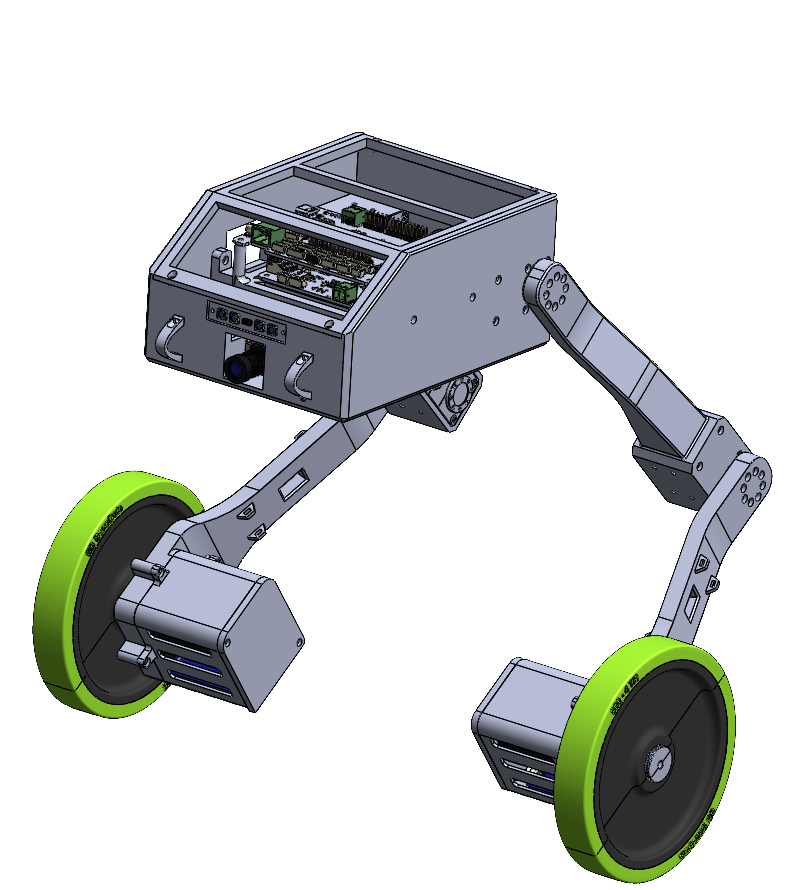
\includegraphics[width = 80mm]{Figures/title/Robot_Assembly_3}
					
					
					\vfill }
		\end{spacing}
	\begin{spacing}{1}
			\begin{tabular}{l}
					\Large{\ArtDerArbeit~\Kennnummer}
					% Die einzutragende Nummer gibt es beim Betreuer!
				\end{tabular}
			
			\vspace{5mm}
			
			\begin{tabular}{l}
					\large{\Autor}\\
					\large{Matrikelnummer \AutorMatrikelNr}
				\end{tabular}
			
			\vspace{5mm}
			
			\begin{tabular}{l}
					\large{Hannover, \Datum}
				\end{tabular}
			
			
			\vspace{5mm}
			{\large
					\begin{tabular}{l l}						
							First Examiner  & \Erstpruefer\\
							Second Examiner & \Zweitpruefer\\
							Supervisor    	& \Betreuer\\
						\end{tabular}
				}
			
		\end{spacing}
\end{titlepage}
%\cleardoublepage

%include Declaration of Authorship
% !TEX encoding = UTF-8 Unicode
% !TEX spellcheck = de_DE
% !TEX root = ../main.tex

\newpage
% Logos oben einbinden
\begin{flushright}
			\vspace*{-20mm}
			
\includegraphics[width=\textwidth]{Figures/title/CoverLogos.pdf}
\end{flushright}
	
\begingroup
\renewcommand{\cleardoublepage}{}
\renewcommand{\clearpage}{}
\chapter*{Declaration of Authorship}
\endgroup
\thispagestyle{empty}

%Kennnummer platzieren:
\begin{tikzpicture}[remember picture, overlay]
\node[xshift=-22mm,yshift=-43mm,anchor=north east,align=right] at (current page.north east){\Large{\textbf{\Kennnummer}}};
\end{tikzpicture}
%
%
\begin{tabular}{@{}p{0.25\textwidth} p{0.7\textwidth}}
\textbf{Name:} 		& \textbf{\Autor} \\ % Name des Autors
Registration no.: & \Matrikelnummer \\ % Matrikelnummer
\\
Thesis title: 		& \TitelDerArbeit \\
\\
Type of thesis: 	& \ArtDerArbeit\\
Study program: 		& International Mechatronics\\ %
%Mechanical Engineering\\ % Please Choose:
Submission date:	& \Datum \\
\\
First examiner : 	& \Erstpruefer\\
Second examiner: 	& \Zweitpruefer\\
Supervisor: 			& \Betreuer
\end{tabular}

\vspace{10mm}

I, \emph{\Autor}, hereby affirm that the \ArtDerArbeit~entitled \emph{\TitelDerArbeit}~was written independently, that no references and aids other than those indicated were used, that all passages of the thesis which were taken over literally or analogously from other sources are marked as such and that the thesis has not yet been presented to any examination board in the same or similar form.

I hereby agree to the transmission of my work also to external services for plagiarism checking by plagiarism software.

\vspace{5mm}


\noindent Hannover, \Datum



\vspace{20mm}
(\Autor)

%\end{spacing}
% Leerseite einfügen
\cleardoublepage

% If desired, include a blank page
\newpage
\thispagestyle{empty}
\mbox{}

% If desired, include a declaration of authorship
\chapter*{Eigenst\"andigkeitserkl\"arung}
\label{cha:Ehrenwort}
\thispagestyle{empty}
Hiermit erkl\"are ich, dass ich die vorliegende Arbeit selbstst\"andig und eigenh\"andig sowie ohne
unerlaubte fremde Hilfe und ausschlie\ss lich unter Verwendung der aufgef\"uhrten Quellen und
Hilfsmittel angefertigt habe.

\vspace{3cm}

\begin{tabular}{lp{4em}l}
 \hspace{4cm}   && \hspace{4cm} \\ \cline{1-1} \cline{3-3} \rule{0pt}{3.5ex} 
 Ort, Datum     && \Autor
\end{tabular}






% Include abstract

\selectlanguage{english}
\begin{abstract}
%General Problem
The robotic industry is growing rapidly.
Robots are becoming more and more capable and are used in a wide range of applications.
The design, modeling and control of robotic systems is a research field that is constantly evolving.

%% Research Gap
However, there are still many challenges to overcome.
The design of robotic systems is still a complex and time-consuming process, particularly in regard to multi-legged robots that should be able to execute complex maneuvers.
The control of robotic systems is still a challenging task, especially when it comes to dynamic and complex systems.
The search for the optimal control strategy is still an open research question.

%% Content
This thesis presents an in-depth exploration of the dynamic control and design of robotic systems.
The main focus is on the design and control of a multi-legged robot.
The robot is designed and built from scratch, including the mechanical and electronic design.
A combination of theoretical modeling and practical implementation were used to achieve the desired objectives.
The research first focuses on the design of a multi-legged robot that is capable of executing complex maneuvers. The robot is then modeled and simulated in a virtual environment.
The simulation is used to test and evaluate the robot's performance.
The robot is then built and tested in real life.
The research investigates the main elements that affect maneuverability and stability, such as the integration of multiple degrees of freedom, structural integrity, and weight distribution.


%% Contributions
Significant results are achieved in the design and control of the robot.
The robot demonstrates the capability to maintain balance while adjusting its hip and knee joint angles, as well as exhibits stable locomotion on its two wheels, effectively navigating within the simulated environment.
The robot's design is optimized to find the best trade-off between stability and maneuverability.
Different problems are addressed throughout the research, such as the design complexity to meet the mobility requirements, Incorporating the changing location of the center of mass in the dynamic model, and retuning the control of the robot when one or both of the joint angles change.
The developed Legged two-wheeled inverted pendulum robot serves as a platform for future research to build upon and test different control strategies.

%Furthermore
This research contributes valuable insights into the field of robotics, offering practical solutions for the challenges faced in designing and controlling wheeled and bipedal robots.
It lays a foundation for future innovations, aiming to broaden the scope and capabilities of robotic systems in real-world applications.




%Overall, this thesis provides a valuable contribution to the field of
%%%
\par
\keywords{Robotics, Multi-Legged Robot, Control, Simulation, Design, CAD, Modeling, Inverted Pendulum, Two-Wheeled bi-pedal legged robot}
\end{abstract}





% If desired, uncomment the table of contents
\tableofcontents

% From the Backmatter --
% If desired, uncomment the list of figures
\listoffigures

% If desired, uncomment the list of tables
\listoftables

% If desired, uncomment the list of listings
%\lstlistoflistings

% Include this switch if symbols, abbreviations, etc., without reference in the document should be included in the directories (usually the case)
% \glsaddall
%\glsaddallunused

%\setglossarypreamble[main]{This list of glossary entries only includes the most important items. Descriptions might not be universal and are intended for this thesis.}

%% If desired, uncomment the glossary (will only be created if entries are available)
%\setglossarystyle{long3col}
%%\setglossarystyle{long}
%\renewenvironment{theglossary}%
% {\begin{longtable}{lp{\glsdescwidth}p{\glspagelistwidth}}}
	% %{\begin{longtable}[l]{lp{\glsdescwidth+\glspagelistwidth+0cm}}}%
		% {\end{longtable}}
	%\renewcommand{\glsnamefont}[1]{\textbf{#1}}
	%\printglossary[type=main, style=altlist]%[style=index]
	%\glsfindwidesttoplevelname
	%\glssetwidest[1]{transfer error dynamics}
	%\setglossarystyle{alttree}
	%\printglossary[type=main]
	
	% If desired, uncomment the abbreviations (will only be created if entries are available)
	%\printglossary[type=\acronymtype, nonumberlist]%[type=\acronymtype,style=list]
	
	% If desired, uncomment the symbols (will only be created if entries are available)
	%\printglossary[type=symbols, style=symb3spaltig, nonumberlist]
	%\printglossary[type=symbols, nonumberlist]
	
	%\chanumfalse
\addchap{Notation} % add chapter without numbering that appears in table of contents
% Manuelles Symbolverzeichnis
% ___________________________________________________________________
% ============================ NOTATION ==========================
% ====================================================================
\begin{table}[h]
	\renewcommand{\arraystretch}{1.4}
	\begin{tabularx}{1\textwidth}{@{}lX@{}}
		\toprule
		\textbf{Example} & \textbf{Description}  \\ \midrule
		$\mathbb{R}, \mathbb{N}$ 	& Capital letters in blackboard bold font represent common number types. \\
		$\mathcal{A}, \mathcal{T}$ 	& Capital letters in calligraphic font represent custom sets or its members. \\
		$\vec{A}, \vec{P}$ 			& Capital bold letters represent matrices.	\\
		$\vec{x}, \vec{f}$			& Lower-case bold letters represent column vectors or vector-functions. \\
		$F(z), T(s)$				& Capital regular letters represent transfer functions.	\\		
		$i, e^{(i \rightarrow j)}$	& Lower-case regular letters represent scalars and scalar-functions.\\
		$\vec{x}^{(i)}, F^{(2)}$	
			& A single upper, bracketed index represents the dependency on a single, specific agent.\\
		$ H^{(1, 2)}, e^{(i, j)}$ 
			& Two upper, bracketed indices represent the dependency on two specific agents, where the order of the agents is not relevant.\\
		$ H^{(1 \rightarrow 2)}, e^{(i \rightarrow j)}$
			& An arrow between two upper, bracketed indices represent the directional dependency on two specific agents, where the order of the agents matters.\\
		$\hat{\vec{t}}^{(i \rightarrow j)}, \hat{\mathbf{P}}^{(1)}$ 
	     	& An upper hat symbol represents an estimated or approximated entity.\\	
		$\bar H^{(1 \rightarrow 2)}, \bar e^{(i \rightarrow j)}$
	     	& An upper bar symbol represents a mean value.\\	
		\bottomrule
	\end{tabularx}
	\caption[General notation style]{General notation style. Some exceptions are possible.}
\end{table}

% ====================================================================
\begin{notebox}
	To be precise, the error dynamics depend on the order of agent $i$ and $j$, 
	since they differ in their sign.
		\begin{equation}
			H^{(i,j)}\neq H^{(j,i)}
		\end{equation}			
		However, both result in the same \gls*{output_error}. 
		$H^{(i,j)}$ and $H^{(j,i)}$ are not distinguished in this work, 
		which is consistent with the given notation. This also applies to other cases like the error trajectory $\vec{e}^{(i,j)}$ or the output error $\varepsilon^{(i,j)}_{\vec{u}}$ as well.
\end{notebox}

% ====================================================================
\pagebreak
\renewcommand{\arraystretch}{1.3}
\begin{tabularx}{1\textwidth}{@{}lX@{}}
    \endfirsthead \endhead \endfoot \endlastfoot
    \toprule
	\multicolumn{2}{@{}l}{\textbf{Mathematical Notations}} \\ 
	\textit{Symbol} & \textit{Description}  \\ \midrule
	$\left\Vert \cdot \right\Vert_2$ & denotes the 2-norm \\
	$\left\Vert \cdot \right\Vert_{\infty}$ & denotes the maximum-norm \\
	$ |\cdot |$	& 
	\begin{enumerate*}[label=(\roman*)]
		\item absolute of a number or 
		\item gain of a transfer function
	\end{enumerate*} \\
	$\angle $ & denotes the phase of a transfer function \\
	$\circ$	& denotes the composition of two functions or matrices \\
	$\vec{0}$ & denotes a zero vector or zero matrix  \\
	$\vec{I}$ & denotes the unit matrix \\
%		$\emptyset$ & denotes an empty set\\
	$\mathcal{N}(\mu, \sigma^2)$& normal distribution with mean $\mu$ and standard deviation $\sigma$ \\ 
	\bottomrule
	\multicolumn{2}{@{}l}{\textbf{General Parameters}} \\ 
	\textit{Symbol} & \textit{Description}  \\ \midrule
	$k, l$		 				&  running indeces \\
	$t$							&  time or duration (in seconds) \\
	$n_{\mathcal{A}}$	 		&  number of agents in a MAS \\
	$N, R$				 		&  dimension of a vector, matrix, i.e. length of an input trajectory \\
	$K$					 		&  degree of a biproper transfer function \\
	$K_N, K_D$		 	 		&	degree of numerator, denominator of a transfer function \\
	$m$						 	&  relative degree of a dynamic system \\
	$f_s, f_\mathrm{cutoff}, f$	&  sample frequency, cutoff frequency, other frequencies in $1/\unit{s}$\\ 
	\bottomrule
	\multicolumn{2}{@{}l}{\textbf{Sets \& Agents}} \\ 
	\textit{Symbol} & \textit{Description}  \\ \midrule
	$i, j$				 &  indices of a specific, but arbitrary agent in a MAS \\
	$\mathbb{R}$		 &	set of all real numbers \\
	$\mathbb{R}^n$		 &	$n$-dimensional set of all real numbers \\
	$\mathbb{N}_0$		 &  set of all natural numbers and zero \\
	$\mathcal{U}^{(i)}$	 	&  input space of agent $i$ \\
	$(\mathcal{U}^{(i)})^N$ &  input space of agent $i$ for input sequences of length $N$\\
	$(\mathcal{U}^{(i,j)})^N$&  input space of agent $i$ and $j$ for input sequences of length $N$ with 
	$(\mathcal{U}^{(i)})^N \cap (\mathcal{U}^{(j)})^N$ \\
    $\mathcal{A}$    	 &  set of all agents in a MAS\\
    $\mathcal{A}^{(i)}$  &  specific agent with index $i$\\
    $\mathcal{T}$    	 &  set of input maps between all agents in a MAS \\
    \bottomrule\\[10mm]\\[0.01mm]    
	\toprule
	\multicolumn{2}{@{}l}{\textbf{Discrete time step $k$}} \\ 
	\textit{Symbol} & \textit{Description}  \\ \midrule
	$k$			 &  time (sample) index for discrete systems and trajectories \\	    
    $u_{k}$		 & scalar input at time step $k$ \\
    $y_{k}$		 & scalar output at time step $k$ \\
   		$e^{(i,j)}_{k}$		 	 
   			& difference $y^{(j)}_k-y^{(j)}_k$ between the outputs of agent $i$ and $j$ at time $k$\\
   		$w_k$
   			& noise drawn from a normal distribution with zero mean and variance $\sigma^2$\\
    $\vec{x}^{(i)}_{k}$  & state of agent $i$ at time $k$ \\	
	$\vec{\tilde{f}}$ 	
		& state-function that advances the state $\vec{x}$ one step in time \\
	$\tilde{h}$ 	
		& output-function that returns the current output depending on the 
		current state and input\\   
	$\vec{A}, \vec{B}, \vec{C}$ 
		& state matrix, input matrix, output matrix of a linear system in discrete-time 
		state-space representation \\ \bottomrule
	\multicolumn{2}{@{}l}{\textbf{Transfer Function Representation}} \\ 
	\textit{Symbol} & \textit{Description}  \\ \midrule
	$s, z$ & denotes a transfer function in continuous time, discrete time\\
	$U(s), U(z)$		
		& System input in $s$-domain, $z$-domain\\
	$E(s), E(z)$		
		& $s$-Transformation, $z$-Transformation of the difference $y^{(j)}-y^{(j)}$\\
	$F$				
		& Transfer function of of a linear system\\
	$F^{(i\rightarrow j)}$	
		& \Glsc{deviation_system} in the transfer-function representation from agent $i$ to agent $j$	\\
	$Q$	
		& Filter function\\	
	$\hat{T}^{(i\rightarrow j)}$	
		& Estimation of the \glsc{input_map} in the transfer-function representation from agent $i$ to agent $j$\\
	$H^{(i,j)}$	
		& \Glsc{error_dynamics} in the transfer function representation describing the difference between agent 
		$i$ and $j$ when the same input is applied to both systems\\
	$H^{(i \rightarrow j)}$	
		& \Glsc{transfer_error_dynamics} in the transfer function representation describing the difference between agent 
		$i$ and $j$ including the input-transfer $\hat T^{(i \rightarrow j)}$\\	
	$a_k, b_k$ & Numerator, denominator coefficients in transfer-function \\ \bottomrule%\\[54mm]\\[0.01mm] \toprule
	\multicolumn{2}{@{}l}{\textbf{Batch Process \& Lifted System Representation}} \\ 
	\textit{Symbol} & \textit{Description}  \\ \midrule
	$\vec{u}, \vec{v}$		  	
		& An \glsc{input_trajectory} as a sequence of scalar inputs of length $N$\\
	$\vec{\tilde u}^{(i)}$	
		& Input trajectory of length $N$ for agent $i$ that results from some input-transfer 
		$\vec{t}^{(j\rightarrow i)}$\\
	$\vec{y}$		 	
		& An \glsc{output_trajectory} as a sequence of scalar outputs of length $N$\\
	$\vec{e}^{(i,j)}$
		& An \glsc{error_trajectory} describing the difference $\vec{y}^{(j)}-\vec{y}^{(i)}$ between the 
		output trajectories of agent $i$ and $j$\\
	$\vec{e}^{(i\rightarrow j)}_{\vec{u}}$
		& \Glsc{transfer_error_trajectory} describing the difference $\vec{y}^{(j)}-\vec{y}^{(i)}$ between the 
		output trajectories of agent $i$ and $j$ for a certain input trajectory $\vec{u}$\\ \midrule\\[0.1mm] \midrule
	\textit{Symbol} & \textit{Description}  \\ \midrule	
	$\vec{w}$
		& Sequence of normally distributed noise values with zero mean and variance $\sigma^2$\\ 	
	$\vec{f}$ 			
		& Nonlinear \glsc{batch_function} that maps a given input trajectory to a corresponding 
		output trajectory \\
	$\vec{f}^{(i\rightarrow j)}$
		& \Glsc{deviation_system} as a \gls*{batch_function} from agent $i$ to agent $j$\\
	$\mathbf{t}^{(i\rightarrow j)}$	
		& \Glsc{input_map} as a \gls*{batch_function} from agent $i$ to agent $j$\\
	$\mathbf{\hat t}^{(i\rightarrow j)}$	
		& Estimated input-transfer batch-function from agent $i$ to agent $j$
		(Here as a general expression for either $\mathbf{\hat T}^{(i\rightarrow j)}$ or $T^{(i\rightarrow j)}$)\\
	$\mathbf{h}^{(i\rightarrow j)}$	
		& \Glsc{error_dynamics} as a \gls*{batch_function} describing the difference between agent 
		$i$ and $j$ when the same input is applied to both systems.\\
	$\vec{P}$				
		& lifted-system matrix that maps an input trajectory to an output trajectory\\
	$\vec{P}^{(i\rightarrow j)}$	
		& \Glsc{deviation_system} in the lifted-system representation from agent $i$ to agent $j$\\
	$\mathbf{T}^{(i\rightarrow j)}$	
		& \Glsc{input_map} in the lifted-system representation from agent $i$ to agent $j$\\
	$p_k, p^{(i \rightarrow j)}_k$					
		& $k$-th parameter in lifted-system matrix $\vec{P}, \vec{P}^{(i\rightarrow j)}$\\
	$t^{(i\rightarrow j)}_k$	
		&  $k$-th parameter in lifted-system matrix $\mathbf{T}^{(i\rightarrow j)}$\\ \bottomrule
	\multicolumn{2}{@{}l}{\textbf{Error Metrics}} \\ 
	\textit{Symbol} & \textit{Description}  \\ \midrule
   		$\varepsilon^{(i,j)}$ % \left(\vec{y}^{(i)}, \vec{y}^{(j)}\right)	 	 
   			& \Glsc{output_error}: 2-norm of the difference between the output trajectories of agent $i$ and $j$\\	
   		$\varepsilon^{(i,j)}_{\vec{u}}$ %\left(\vec{u}^{(i)}\right)		 	 
   			& \Glsc{direct_transfer_error}: Output error $e^{(i,j)}$ when the same input is applied 
   			to agents $i$ and $j$ \\
	$\varepsilon^{(i\rightarrow j)}_{\vec{u}}$ 
		& \Glsc{transfer_error}: Output error $\varepsilon^{(i,j)}$  for a certain input trajectory $\vec{u}$ 
			after applying the \gls*{input_map} $\vec{t}^{(i \rightarrow j)}$ to agent $j$ \\	
	$\varepsilon^{(i\rightarrow j)}_{\vec{u},\mathrm{NRMS}}$ 
		& \Glsc{nte}: Transfer error $\varepsilon^{(i\rightarrow j)}_{\vec{u}}$ 
		normalized to the \gls*{direct_transfer_error} $\varepsilon^{(i,j)}_{\vec{u}}$\\	
	\bottomrule
	\caption{Mathematical notations}
\end{tabularx}

\chanumtrue
    
	% --
	
	% Save page number for Back Matter and conclude Front Matter
\newcounter{RomanNumbers}
\addtocounter{RomanNumbers}{\value{page}}
\clearpage
